\documentclass[]{book}
\usepackage{lmodern}
\usepackage{amssymb,amsmath}
\usepackage{ifxetex,ifluatex}
\usepackage{fixltx2e} % provides \textsubscript
\ifnum 0\ifxetex 1\fi\ifluatex 1\fi=0 % if pdftex
  \usepackage[T1]{fontenc}
  \usepackage[utf8]{inputenc}
\else % if luatex or xelatex
  \ifxetex
    \usepackage{mathspec}
  \else
    \usepackage{fontspec}
  \fi
  \defaultfontfeatures{Ligatures=TeX,Scale=MatchLowercase}
\fi
% use upquote if available, for straight quotes in verbatim environments
\IfFileExists{upquote.sty}{\usepackage{upquote}}{}
% use microtype if available
\IfFileExists{microtype.sty}{%
\usepackage{microtype}
\UseMicrotypeSet[protrusion]{basicmath} % disable protrusion for tt fonts
}{}
\usepackage[margin=1in]{geometry}
\usepackage{hyperref}
\hypersetup{unicode=true,
            pdftitle={Leefomstandigheden inwoners met een Antilliaanse achter-grond in Den Haag},
            pdfauthor={Esther Horrevorts,Hans Bellaart},
            pdfborder={0 0 0},
            breaklinks=true}
\urlstyle{same}  % don't use monospace font for urls
\usepackage{natbib}
\bibliographystyle{apalike}
\usepackage{longtable,booktabs}
\usepackage{graphicx,grffile}
\makeatletter
\def\maxwidth{\ifdim\Gin@nat@width>\linewidth\linewidth\else\Gin@nat@width\fi}
\def\maxheight{\ifdim\Gin@nat@height>\textheight\textheight\else\Gin@nat@height\fi}
\makeatother
% Scale images if necessary, so that they will not overflow the page
% margins by default, and it is still possible to overwrite the defaults
% using explicit options in \includegraphics[width, height, ...]{}
\setkeys{Gin}{width=\maxwidth,height=\maxheight,keepaspectratio}
\IfFileExists{parskip.sty}{%
\usepackage{parskip}
}{% else
\setlength{\parindent}{0pt}
\setlength{\parskip}{6pt plus 2pt minus 1pt}
}
\setlength{\emergencystretch}{3em}  % prevent overfull lines
\providecommand{\tightlist}{%
  \setlength{\itemsep}{0pt}\setlength{\parskip}{0pt}}
\setcounter{secnumdepth}{5}
% Redefines (sub)paragraphs to behave more like sections
\ifx\paragraph\undefined\else
\let\oldparagraph\paragraph
\renewcommand{\paragraph}[1]{\oldparagraph{#1}\mbox{}}
\fi
\ifx\subparagraph\undefined\else
\let\oldsubparagraph\subparagraph
\renewcommand{\subparagraph}[1]{\oldsubparagraph{#1}\mbox{}}
\fi

%%% Use protect on footnotes to avoid problems with footnotes in titles
\let\rmarkdownfootnote\footnote%
\def\footnote{\protect\rmarkdownfootnote}

%%% Change title format to be more compact
\usepackage{titling}

% Create subtitle command for use in maketitle
\newcommand{\subtitle}[1]{
  \posttitle{
    \begin{center}\large#1\end{center}
    }
}

\setlength{\droptitle}{-2em}

  \title{Leefomstandigheden inwoners met een Antilliaanse achter-grond in Den
Haag}
    \pretitle{\vspace{\droptitle}\centering\huge}
  \posttitle{\par}
    \author{Esther Horrevorts,Hans Bellaart}
    \preauthor{\centering\large\emph}
  \postauthor{\par}
      \predate{\centering\large\emph}
  \postdate{\par}
    \date{September 2018}

\usepackage{booktabs}
\usepackage{booktabs}
\usepackage{longtable}
\usepackage{array}
\usepackage{multirow}
\usepackage[table]{xcolor}
\usepackage{wrapfig}
\usepackage{float}
\usepackage{colortbl}
\usepackage{pdflscape}
\usepackage{tabu}
\usepackage{threeparttable}
\usepackage{threeparttablex}
\usepackage[normalem]{ulem}
\usepackage{makecell}

\begin{document}
\maketitle

{
\setcounter{tocdepth}{1}
\tableofcontents
}
\hypertarget{inleiding}{%
\chapter*{Inleiding}\label{inleiding}}
\addcontentsline{toc}{chapter}{Inleiding}

In een eerdere publicatie van Kennisplatform Integratie \& Samenleving
kwam een zorgelijk beeld naar voren van de leefomstandigheden van
kinderen met een Antilliaanse- of Arubaanse achter-grond in Nederland
\citep{Tierolf2017}.

Het was opvallend dat kinderen met een Antilliaanse achtergrond,
vergeleken met jeugd van ande-re herkomst, het hoogst scoren op de
risico's op armoede, eenoudergezinnen, jeugdwerkloosheid en gebruik
jeugdhulp. Er zijn grote verschillen in de leefomstandigheden waarin
kinderen zonder en met een migratieachtergrond opgroeien. Het maakt uit
in welke wijk je opgroeit. Jeugdigen met een Antilliaanse achtergrond
wonen vaker in de slechtere, kansarme wijken en voelen zich daar minder
veilig. Ondanks de gemiddelde slechtere leefomstandigheden doet een deel
van de Antilli-aanse jongeren het wel goed in het onderwijs en op de
arbeidsmarkt. Het opleidingsniveau van deze jongeren stijgt gestaag,
maar al met al is het beeld dat de leefomstandigheden van een rela-tief
groot deel van de inwoners met een Antilliaanse achtergrond niet zo
rooskleurig zijn.

Actieve organisaties voor en door Antilliaanse Nederlanders in Den Haag,
HAAB en OCAN hebben Kennisplatform Integratie \& Samenleving verzocht om
de situatie in Den Haag in kaart te brengen. Dit zou kunnen dienen als
een voorbeeld voor andere gemeenten. Deze organisaties willen graag meer
inzicht krijgen in de specifieke problemen en de kansen om daar nieuwe
projecten voor te ontwikkelen. Zij willen als zelforganisaties zich
versterken en samen met anderen de maatschappe-lijke situatie van veel
Antilliaanse Nederlanders verbeteren.

Voorliggend factsheet hoopt aan de vraag van HAAB en OCAN te voldoen. Op
een groot aantal thema's zijn kerncijfers verzameld. Bij ieder beeld
wordt uitleg gegeven en een korte verklaring van de mate waarin de
cijfers van bepaalde groepen verschillen van elkaar en van het
gemiddelde in Nederland.

\hypertarget{antilliaanse-nederlanders-in-den-haag}{%
\chapter*{Antilliaanse Nederlanders in Den
Haag}\label{antilliaanse-nederlanders-in-den-haag}}
\addcontentsline{toc}{chapter}{Antilliaanse Nederlanders in Den Haag}

\textbf{Inwoners Nederland}\\
Nederland telt in 2017 17.081.507 inwoners. Veruit de grootste groep
inwoners heeft een Neder-landse achtergrond (77,4\%), gevolgd door de
groep westerse migranten (9,9\%). Met een aantal van ruim 150.000
inwoners, vormen de Antilliaans-Nederlandse inwoners een kleine groep in
Neder-land (0,9\%).

\begin{figure}
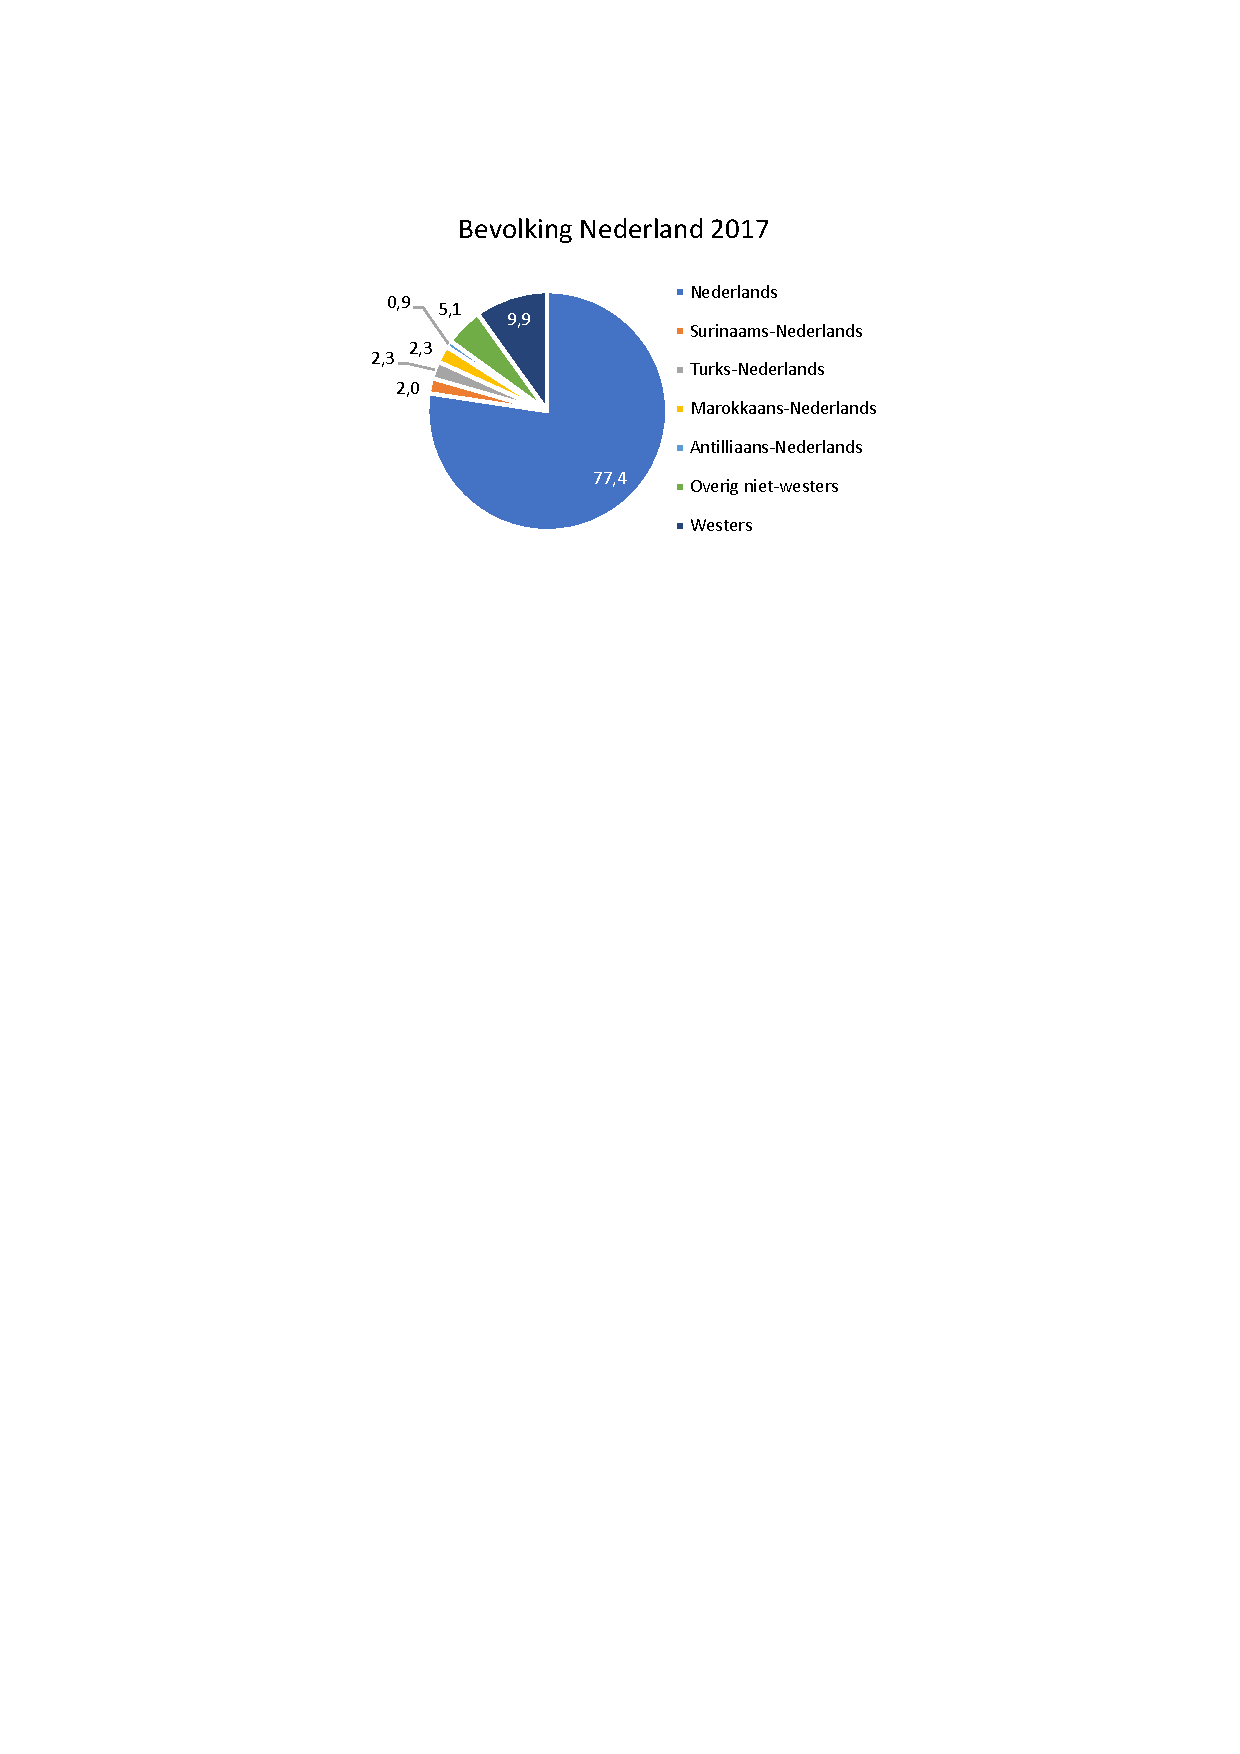
\includegraphics[width=11.32in]{H:/DenHaag/Boek/DenHaag/img/Fig1} \caption{Bevolking Nederland}\label{fig:unnamed-chunk-1}
\end{figure}

\textbf{Inwoners Den Haag}\\
Het aantal inwoners met een Antilliaanse achtergrond in Den Haag is
hoger dan gemiddeld in Nederland. In 2017 telt Den Haag 525.882
inwoners. Daarvan hebben 12.741 inwoners een Antilliaanse achtergrond
(2,4\%).

\begin{figure}
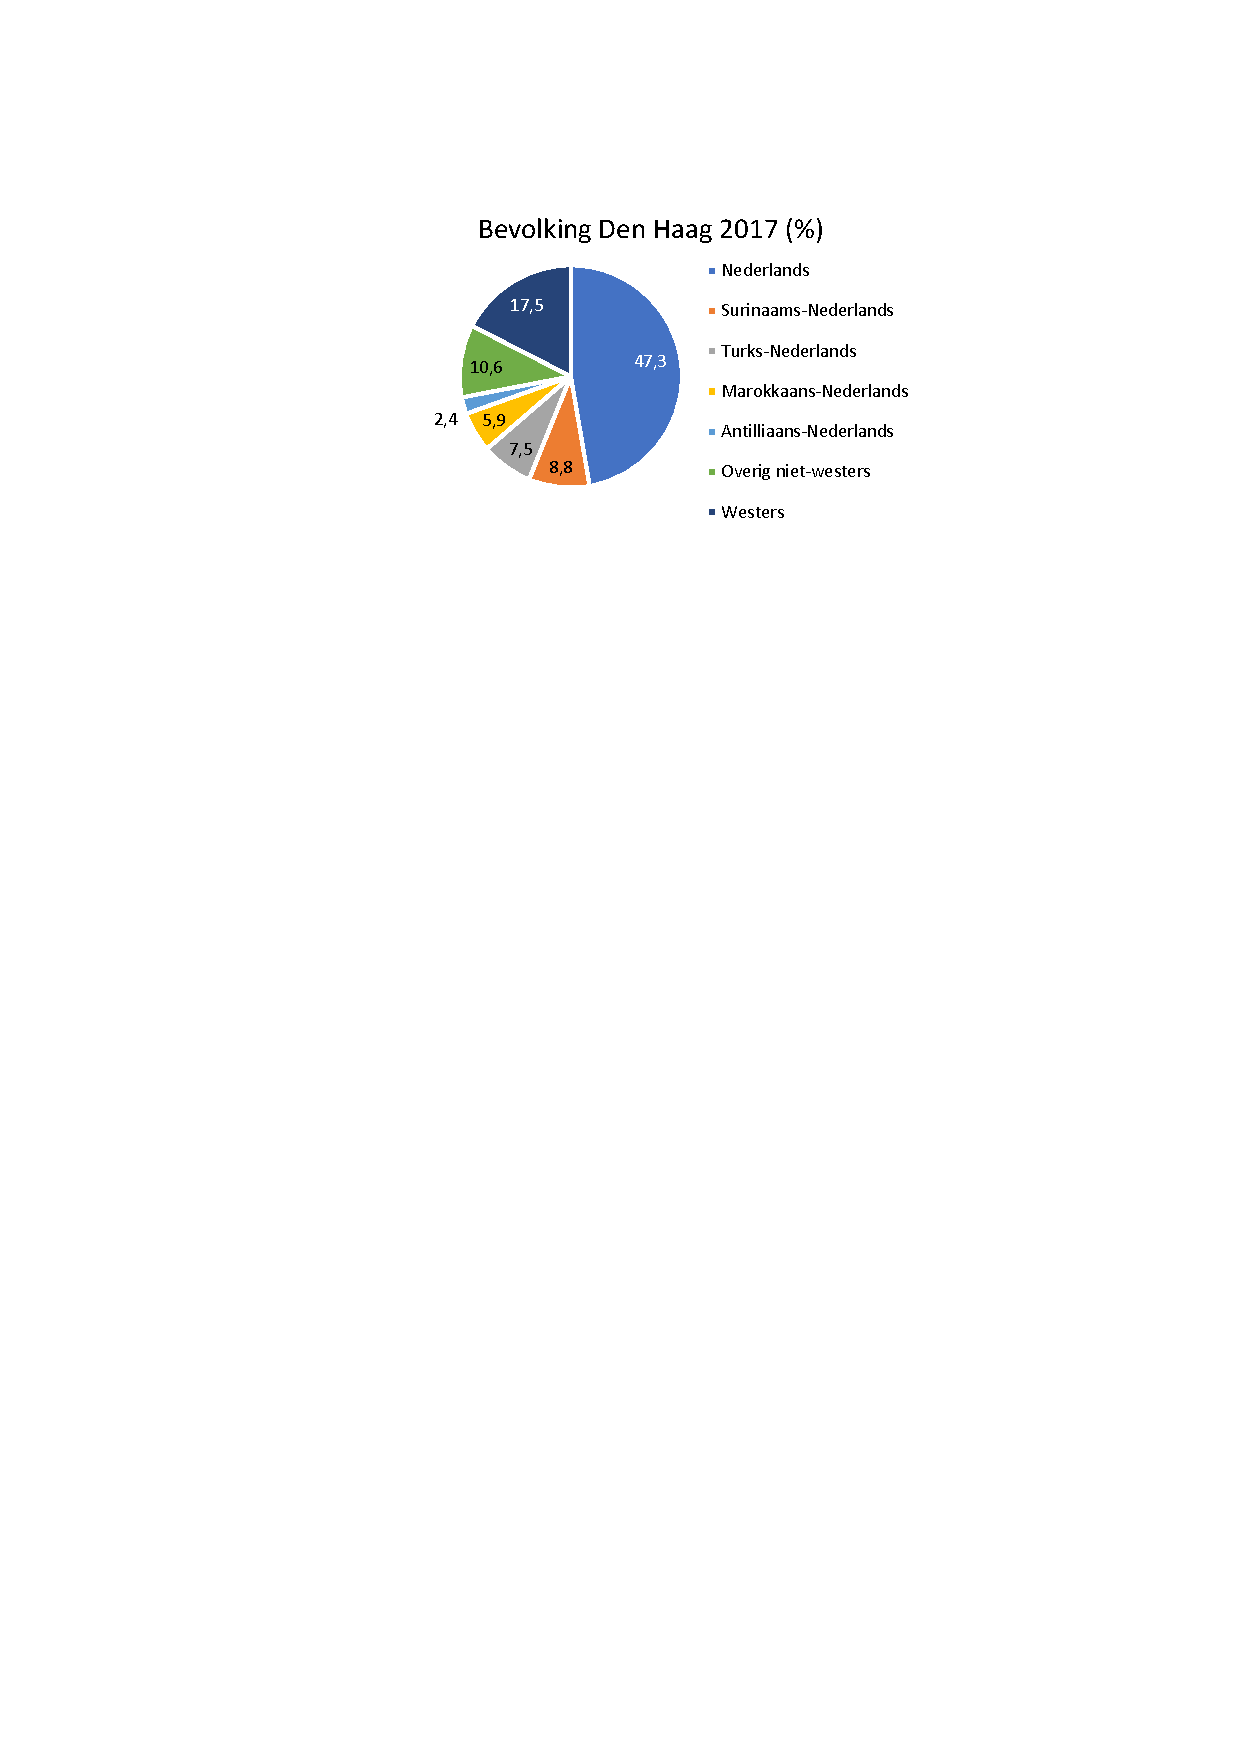
\includegraphics[width=10.33in]{H:/DenHaag/Boek/DenHaag/img/Fig2} \caption{Bevolking Den Haag}\label{fig:unnamed-chunk-2}
\end{figure}

\textbf{Vergelijking G4-steden}\\
Van de andere drie grote steden (Amsterdam, Rotterdam en Utrecht) heeft
Rotterdam ook relatief een grote populatie Antilliaans-Nederlandse
inwoners. Van alle Rotterdamse inwoners, heeft 3,9\% een Antilliaanse
achtergrond. In Amsterdam heeft 1,5\% een Antilliaanse achtergrond en in
Utrecht slechts 0,8\%.

\textbf{Verdeling naar wijken in Den Haag}\\
Wanneer we kijken naar wijkniveau, zijn daar ook grote verschillen in te
zien. De wijk Binckhorst is de wijk met relatief het hoogste aantal
Antilliaans-Nederlandse inwoners (12,1\%). Dit is echter ook een kleine
wijk, waardoor percentages snel hoog uitvallen. Kijken we naar absolute
aantallen, dan hebben de wijken Stationsbuurt (8,4\%), Laakkwartier
(4,8\%) en Moerwijk (4,8\%) het hoogste aan-tal Antilliaans-Nederlandse
inwoners \{\citet{Haag2017}{]}.

\begin{figure}
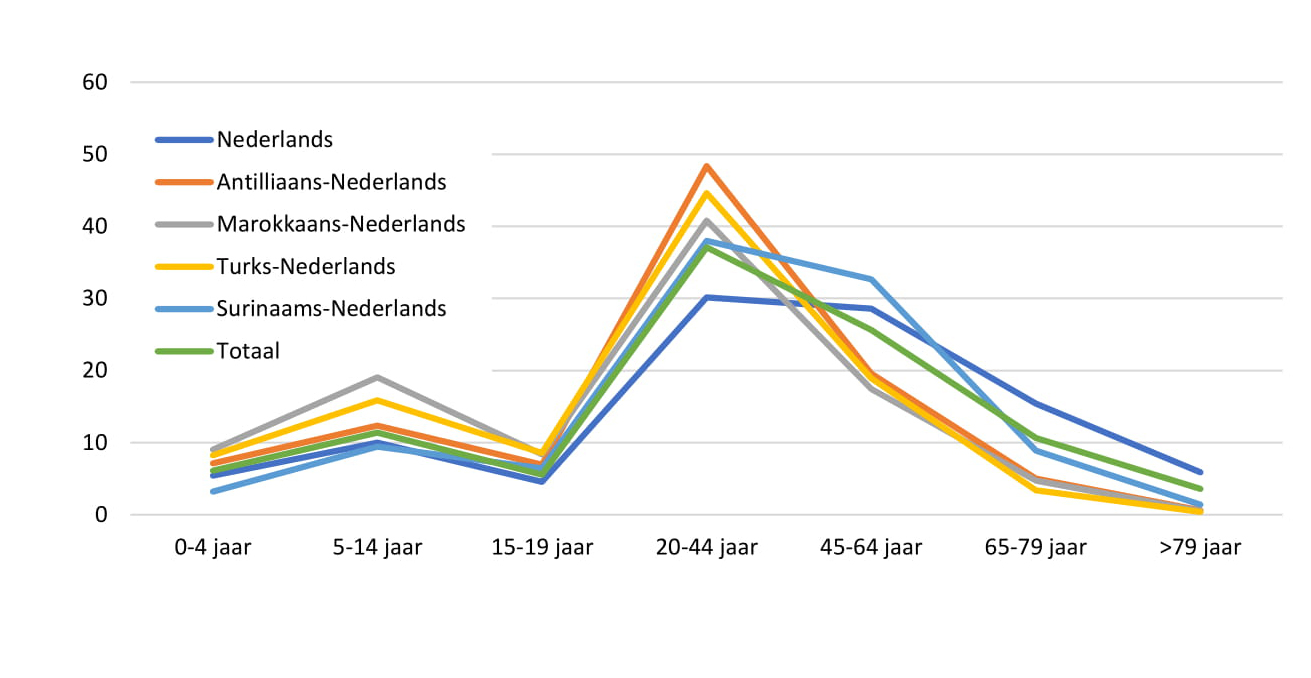
\includegraphics[width=18.21in]{H:/DenHaag/Boek/DenHaag/img/Fig3} \caption{Leeftijdsopbouw inwoners Den Haag}\label{fig:unnamed-chunk-3}
\end{figure}

\textbf{Leeftijdsopbouw}\\
In Den Haag valt de grootste groep inwoners in de leeftijdscategorie
20-44 jaar (37\%). Bijna de helft van de Antilliaans-Nederlandse
inwoners is tussen de 20-44 jaar oud. Bij de inwoners met een
Ne-derlandse achtergrond ligt dit percentage rond de 30\%. Het aantal
kinderen en jeugdigen (0-19 jaar) van inwoners met een Antilliaanse
achtergrond volgt de lijn van het totale aantal inwoners in Den Haag.
Het aantal ouderen is echter weer lager dan gemiddeld. Ditzelfde geldt
ook voor oudere inwoners met een Marokkaanse of Turkse achtergrond.

\begin{table}

\caption{\label{tab:table-aligned}Percentage eenoudergezinnen Den Haag en Rotterdam, 2017}
\centering
\begin{tabular}[t]{l|l|l}
\hline
Achtergronden & Den Haag & Rotterdam\\
\hline
Nederlands & 6,9 & 6,1\\
\hline
Surinaams-Nederlands & 18,1 & 22,3\\
\hline
Antilliaans-Nederlands & 17,2 & 23,9\\
\hline
Turks-Nederlands & 13,1 & 13,7\\
\hline
Marokkaans-Nederlands & 12,2 & 15,2\\
\hline
Overig niet-westers & 11,9 & 13,6\\
\hline
Westers & 7,3 & 8,7\\
\hline
Totaal & 9,4 & 10,6\\
\hline
\end{tabular}
\end{table}

\textbf{Eenoudergezinnen}\\
Het aantal eenoudergezinnen in Den Haag is onder inwoners met een
migratieachtergrond het hoogst. Inwoners met een Surinaamse en
Antilliaanse achtergrond hebben het hoogste percenta-ge ??noudergezinnen
(18,1\% en 17,2\%). Gemiddeld ligt dit percentage in Den Haag een stuk
lager, op 9,4\%. Ook Rotterdam, een stad met tevens relatief veel
Antilliaanse-Nederlanders, heeft een hoog percentage eenoudergezinnen
onder de inwoners met een migratieachtergrond. En ook hier valt op dat
het percentage ??noudergezinnen het hoogst is onder de inwoners met een
Antilliaan-se of Surinaamse achtergrond (23,9\% en 22,3\%
respectievelijk).

\textbf{Mogelijke verklaringen} Het feit dat eenoudergezinnen veelvuldig
voorkomen bij gezinnen met een Antilliaanse achter-grond, kan verklaard
worden door de man-vrouw relatie in Antilliaanse gezinnen. Zo heeft het
krijgen van kinderen onder Antillianen historisch gezien geen sterke
koppeling met samenwonen of trouwen in vergelijking tot gezinnen met een
Nederlandse achtergrond \citep{Distelbrink2011}. Een tweeoudergezin is
voor velen wel een ideaal, maar ? met name in de lagere klasse ? wordt
dat niet altijd gerealiseerd. Deels staan moeders ervan begin af aan al
alleen voor en kiezen ze er ook minder snel voor om, nadat ze uit elkaar
zijn gegaan, opnieuw te gaan samenwonen met een nieuwe partner
\citep{Distelbrink2000}.

\hypertarget{opleidingsniveau-en-onderwijs}{%
\chapter*{Opleidingsniveau en
Onderwijs}\label{opleidingsniveau-en-onderwijs}}
\addcontentsline{toc}{chapter}{Opleidingsniveau en Onderwijs}

\textbf{Opleidingsniveau Den Haag}\\
Onder alle inwoners van Den Haag heeft 45\% een hoog, 31\% een
middelbaar en 24\% een laag op-leidingsniveau. Hier zitten echter
verschillen in naar herkomstgroep. Van de Antilliaans-Nederlandse
inwoners heeft bijna de helft een middelbaar opleidingsniveau en ruim
een kwart een hoog opleidingsniveau. Inwoners met een Marokkaanse en
Turkse achtergrond hebben het hoogste aandeel met een laag
opleidingsniveau (45\% en 46\%). Inwoners met een Nederlandse of
westerse achtergrond hebben het hoogste aandeel met een hoog
opleidingsniveau (52\% en 57\%).

\begin{figure}
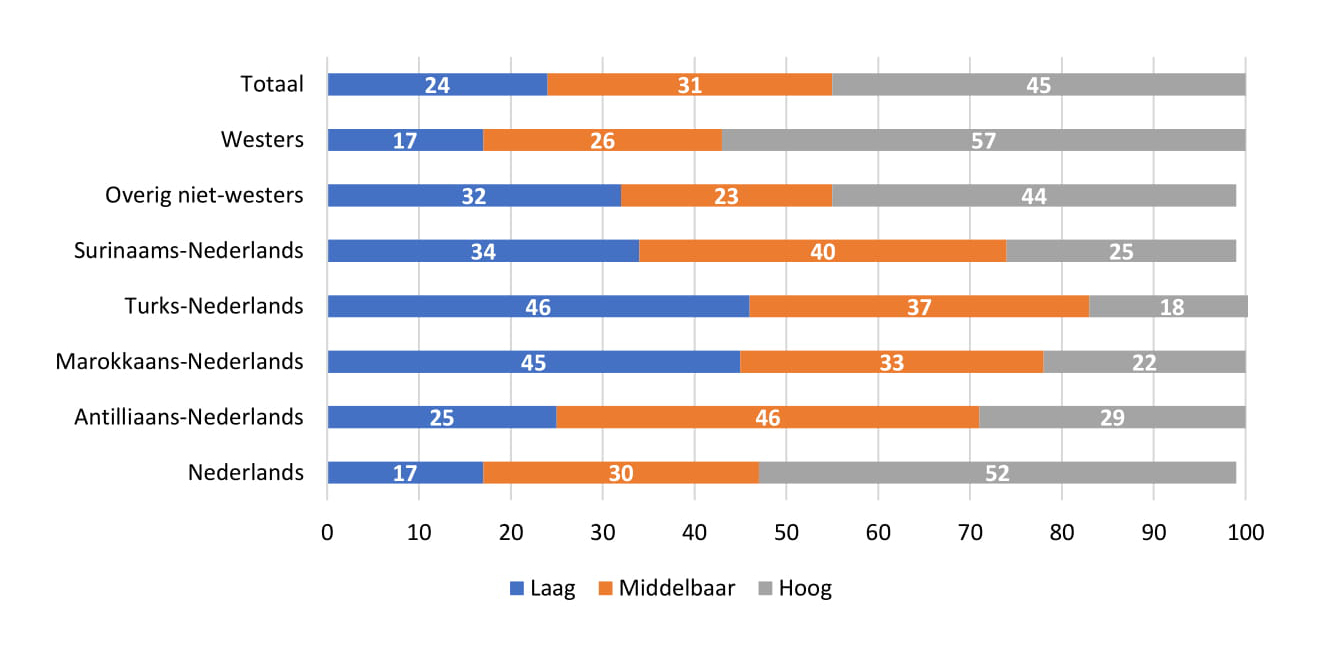
\includegraphics[width=18.46in]{H:/DenHaag/Boek/DenHaag/img/Fig4} \caption{Opleidingsniveau naar herkomst Den Haag, 2013}\label{fig:unnamed-chunk-4}
\end{figure}

\textbf{Opleidingsniveau Nederland} Ook in Nederland heeft bijna de
helft van de Antilliaanse-Nederlanders een middelbaar oplei-dingsniveau
(46\%). Dit komt overeen met de cijfers in Den Haag. Een verschil is dat
landelijk gezien een derde van de inwoners met een Antilliaanse
achtergrond een laag opleidingsniveau heeft, en ongeveer een vijfde een
hoog opleidingsniveau. In Den Haag heeft een kwart een laag
opleidings-niveau en ongeveer een derde juist een hoog opleidingsniveau.

\begin{figure}
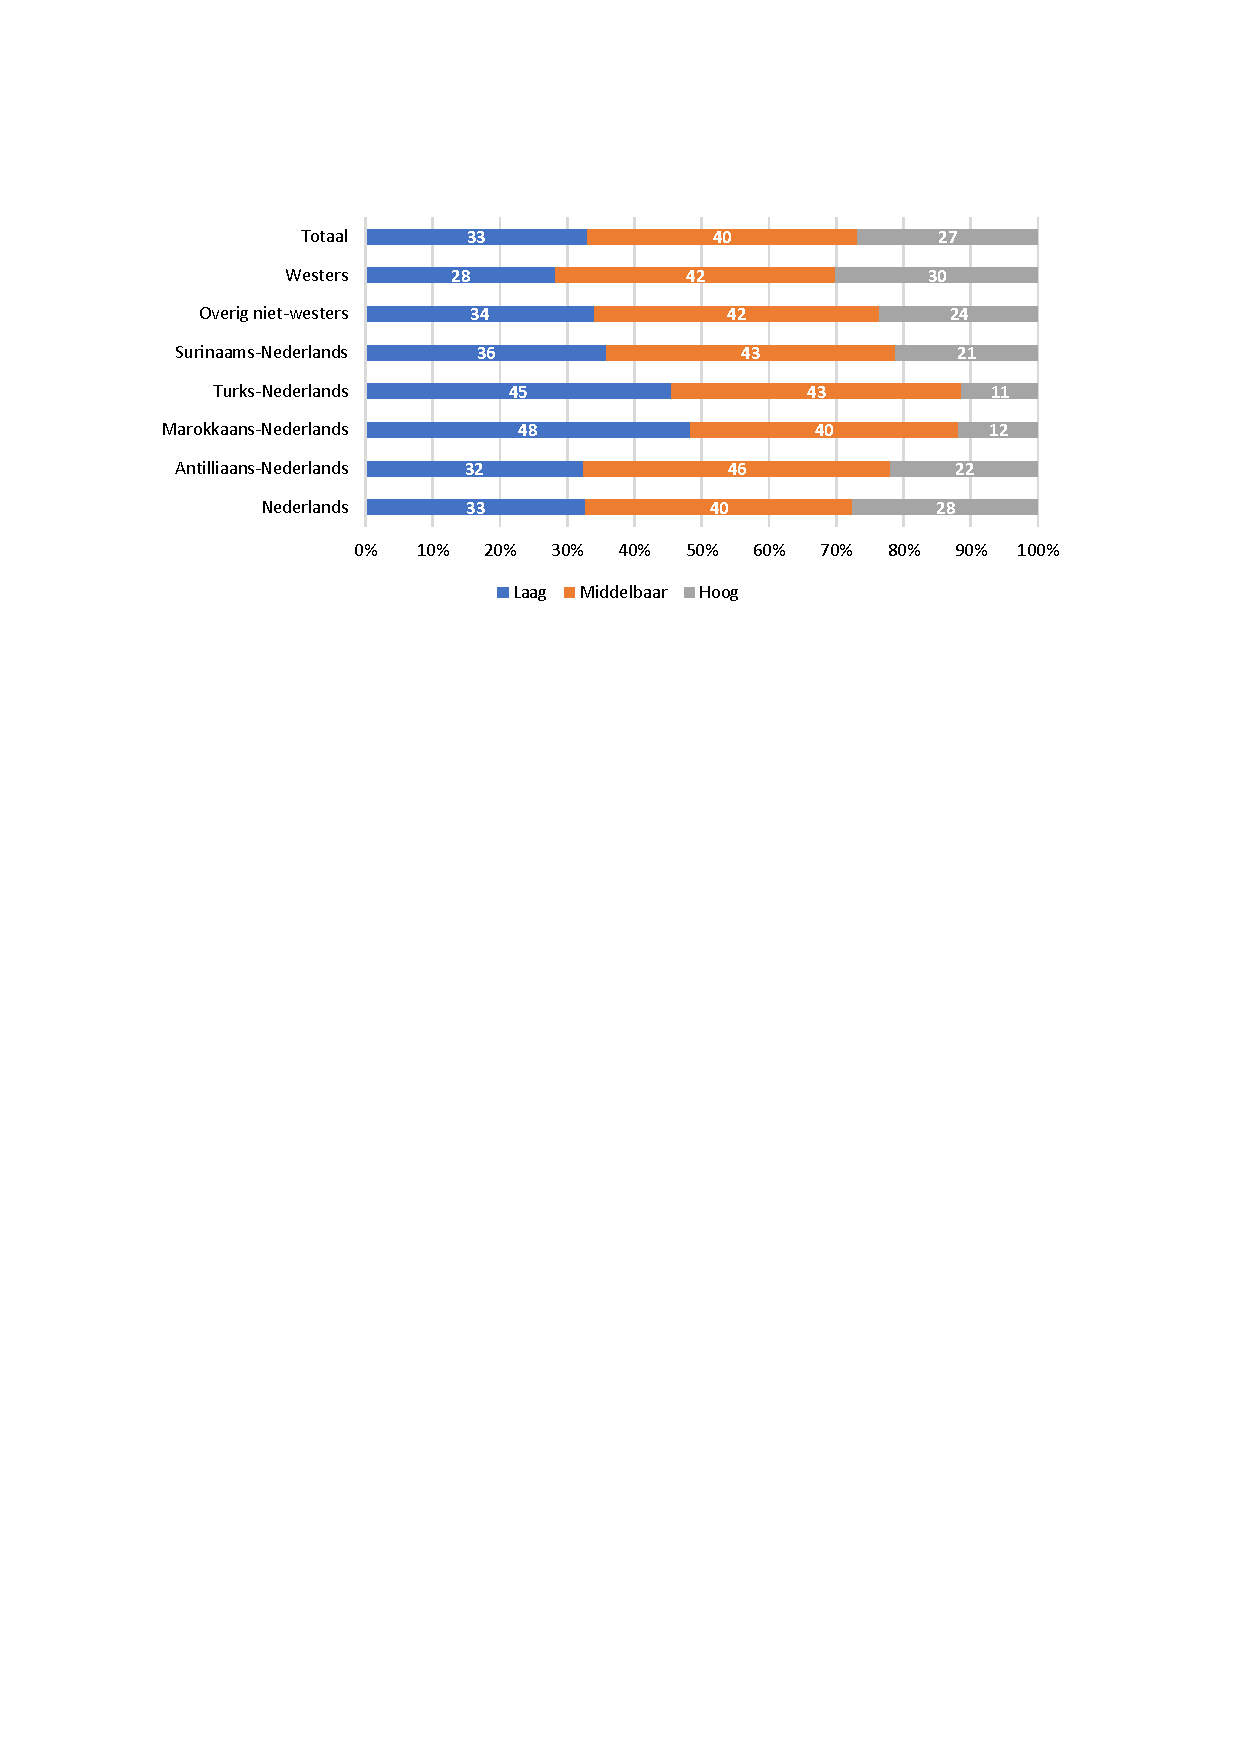
\includegraphics[width=17.89in]{H:/DenHaag/Boek/DenHaag/img/Fig5} \caption{Opleidingsniveau naar herkomst Nederland, 2013}\label{fig:unnamed-chunk-5}
\end{figure}

\textbf{Voortijdig Schoolverlaten}\\
Het schooljaar 2011-2012 telde in totaal 1.600 vroegtijdige
schoolverlaters (VSV-ers) in Den Haag, wat neerkomt op een gemiddelde
van 4,9\%. Het grootste percentage schoolverlaters is onder jon-geren
met een Antilliaanse achtergrond (9,2\%). Rotterdam heeft in 2014 een
iets hoger percentage VSV-ers (5,4\%), en ook hier hebben de
Antilliaans-Nederlandse scholieren het hoogste percentage VSV-ers
(7,4\%).

\begin{table}

\caption{\label{tab:unnamed-chunk-6}Voortijdige Schoolverlaters Den Haag (2011-2012) en Rotterdam (2014}
\centering
\begin{tabular}[t]{l|l|l|l|l}
\hline
Achtergronden & n & \% & n & \%\\
\hline
Nederlands & 545 & 4,0 & 1657 & 5,1\\
\hline
Antilliaans-Nederlands & 104 & 9,2 & 358 & 7,4\\
\hline
Marokkaans-Nederlands & 187 & 5,7 & 517 & 6,1\\
\hline
Turks-Nederlands & 228 & 5,4 & 645 & 6,9\\
\hline
Surinaams-Nederlands & 203 & 4,8 & 516 & 6,3\\
\hline
Overig niet-westers & 172 & 4,8 & 375 & 4,8\\
\hline
Westers & 161 & 5,7 & 351 & 4,5\\
\hline
Totaal & 1600 & 4,9 & 4419 & 5,4\\
\hline
\end{tabular}
\end{table}

\textbf{Mogelijke verklaringen} Leerlingen met een migratieachtergrond
verlaten school vaker vroegtijdig dan leerlingen met een Nederlandse
achtergrond. Dit geldt met name voor jongeren met een Antilliaanse
achtergrond. Vaak zijn deze jongeren hun onderwijsloopbaan al gestart
met een taalachterstand, doordat zij de Nederlandse taal onvoldoende
beheersen (Meeng, 2008) en deze ook niet altijd thuis gesproken wordt
(Holter, 2014). Deze achterstanden worden tijdens hun onderwijsloopbaan
onvoldoende ingelopen, waardoor zij groter risico hebben op vroegtijdig
schoolverlaten \citep{Meeng2008}.

Ook de samenstelling van het gezin vormt een risicofactor. Zo lopen
kinderen uit eenoudergezin-nen meer risico op voortijdig schoolverlaten
\citep{Traag2008}. De verklaring die hier-voor wordt gegeven is dat
kinderen uit eenoudergezinnen minder sociale interactie hebben,
aangezien maar een ouder beschikbaar is. Dit betekent dat deze kinderen
minder van de hulpbronnen van hun ouders kunnen profiteren, wat de kans
op schoolverlaten vergroot. En zoals ook blijkt uit hoofdstuk 2, zijn er
relatief veel eenoudergezinnen onder Antilliaanse-Nederlanders.

\hypertarget{werk-en-inkomen}{%
\chapter*{Werk en inkomen}\label{werk-en-inkomen}}
\addcontentsline{toc}{chapter}{Werk en inkomen}

\textbf{Werkzoekenden en uitkeringsgerechtigden in Den Haag}\\
In Den Haag is 7,1\% van de beroepsbevolking tussen de 15 en 64 jaar
werkzoekend. Het hoogste percentage werkzoekenden zien we terug bij de
inwoners met een Marokkaanse en Antilliaanse achtergrond
(respectievelijk 12,9\% en 12,4\%) (tabel 2).

Ook het aandeel uitkeringsgerechtigden in de leeftijdscategorie 15-64
jaar is onder Antilliaans-Nederlandse inwoners hoog. Onder de jongere
inwoners (15-24 jaar) in Den Haag is gemiddeld 2,3\%
uitkeringsgerechtigd. Bij Antilliaans-Nederlandse inwoners ligt dit op
4,2\%. Kijken we in figuur 2 naar de ouderen (55-64 jaar) dan is het
verschil ten opzichte van het gemiddelde nog veel groter (9,8\% om
26,3\%).

\textbf{Aantal minimahuishoudens Den Haag}\\
In 2011 zijn er in totaal 43.810 huishoudens in Den Haag met een inkomen
tot maximaal 110\% van het wettelijk sociaal minimumloon (WSM). Ruim een
derde van deze huishoudens, bestaat uit per-sonen met een
migratieachtergrond. Kijken we naar cijfers van de herkomst van inwoners
van Den Haag, dan valt op dat inwoners met een niet-westerse achtergrond
oververtegenwoordigd zijn in de minimahuishoudens, dan je op basis van
hun aandeel in de bevolking mag verwachten. Van alle inwoners in Den
Haag heeft 2,4\% een Antilliaanse achtergrond. Echter vormen zij 5\% van
de mini-mahuishoudens.

\textbf{Aantal kinderen in minimahuishoudens in Den Haag}\\
In 2015 groeiden 23.857 kinderen in Den Haag op in een minimahuishouden.
Hierover zijn echter geen cijfers beschikbaar naar herkomst. Kijken we
naar cijfers uit 2011, dan groeiden 22.000 kin-deren op in een
minimahuishouden, waarvan 18.000 kinderen met een migratieachtergrond
(82\%). Uitgesplitst naar herkomst, valt op dat van alle
Marokkaans-Nederlandse kinderen 53\% opgroeit in een minimahuishouden,
bij Antilliaans-Nederlandse kinderen is dat 42\%, bij Turks-Nederlandse
kinderen 33\%, bij Surinaams-Nederlandse kinderen 20\% en bij kinderen
met een Nederlandse ach-tergrond groeit 9\% op in een minimahuishouden.
Over alle kinderen gemiddeld genomen, groeit 21\% op in een
minimahuishouden.

\textbf{Minimahuishoudens in Amsterdam}\\
De trend die in Den Haag zichtbaar is, is ook te zien in Amsterdam. Ook
in Amsterdam zijn de huis-houdens met een maximaal inkomen tot 120\% WSM
{[}\^{}1{]}:(In Amsterdam zijn geen cijfers beschikbaar over
minimahuishoudens met een maximaal inkomen tot 110\% WSM. Andersom zijn
er in Den Haag geen cijfers beschikbaar over minimahuishoudens met een
maximaal inko-men tot 120\% WSM.) oververtegenwoordigd door inwoners met
een niet-westerse achtergrond (55\%). Van alle minimahuishoudens in
Amsterdam, heeft 1,9\% een Antilliaanse achtergrond. Dit staat ongeveer
gelijk aan hun aandeel in de Amsterdamse bevolking (1,5\%). Van de
andere inwoners met een niet-westerse achtergrond, is het aandeel in de
minima-huishoudens hoger dan je op basis van hun aandeel in de
Amsterdamse bevolking zou mogen ver-wachten.

Wanneer gekeken wordt naar de armoedekans (het aandeel van een bepaalde
herkomstgroep dat leeft in een huishouden tot maximaal 120\% WSM, ten
opzichte van die hele herkomstgroep) hebben Marokkaanse-Nederlanders
(34\%), Turkse-Nederlanders (32\%) en inwoners met een overige
niet-westerse achtergrond (36\%) de grootste kans om in armoede te
leven. Van de Antilliaanse-Nederlanders in Amsterdam leeft 28\% in een
huishouden tot maximaal 120\% WSM.

\textbf{Mogelijke verklaringen}\\
Het verschil in werkloosheidscijfers van Antillianen ten opzichte van
autochtonen kan voor een deel verklaard worden doordat ze een lager
opleidingsniveau hebben (Andriessen et al., 2007). Ook een onvoldoende
beheersing van de Nederlandse taal kan bijdragen aan een slechtere
positie op de arbeidsmarkt (Meeng, 2008). Daarnaast kan discriminatie
ook een rol spelen. Zo geeft 19\% van de niet-werkenden met een
Antilliaanse achtergrond aan dat discriminatie de belangrijkste reden is
waarom zij een minder goede kans hebben op een baan dan een inwoner met
een Neder-landse achtergrond die dezelfde opleiding en werkervaring
heeft \citep{Andriessen2007}.

Het relatief hoog aantal uitkeringsgerechtigden onder
Antilliaanse-Nederlanders hangt dan ook weer samen met de hoge
werkloosheidscijfers onder Antilliaanse-Nederlanders. Daarnaast heb-ben
alleenstaanden ook vaker recht op een uitkering dan mensen die een
huishouden delen met andere volwassenen. Voor de
Antilliaanse-Nederlanders is dit een belangrijke verklaring voor het
verschil in uitkering in vergelijking met inwoners met een Nederlandse
achtergrond \citep{Huijnk2013}. Immers, onder Antilliaanse-Nederlanders
zijn relatief veel eenoudergezinnen, zoals blijkt uit Hoofdstuk 2.

\hypertarget{zorggebruik-algemeen}{%
\chapter*{Zorggebruik algemeen}\label{zorggebruik-algemeen}}
\addcontentsline{toc}{chapter}{Zorggebruik algemeen}

\textbf{Zorggebruik onder Haagse inwoners}\\
Uit literatuur blijkt dat het aanbod en de werkwijze binnen de
Nederlandse gezondheidszorg niet altijd goed aansluit op de behoeften
van mensen met een migratieachtergrond. In Den Haag is daarom in 2016
een onderzoek uitgevoerd door het Verwey-Jonker Instituut naar het
gebruik van verschillende vormen van zorg onder de Haagse inwoners
\citep{Hamdi2017}. In het onderzoek, uitgevoerd door Hamdi e.a. (2017),
is een verschil zichtbaar tussen het gebruik van huisartsen- en
ziekenhuiszorg enerzijds, en de thuiszorg, GGZ en ouderenzorg
ander-zijds.

\textbf{Oververtegenwoordiging}\\
\emph{Huisartsenzorg} Van de Haagse inwoners met een Antilliaanse
achtergrond heeft 83\% in het afgelopen jaar de huisarts minimaal 1 keer
bezocht. Hiermee zijn zij samen met inwoners met een Marokkaanse
achtergrond de hoogste gebruikers van huisartsenzorg. Bij inwoners met
een Turkse en Surinaamse achtergrond ligt dit op 80\%. Bij inwoners met
een Nederlandse achtergrond heeft 77\% de huisarts minimaal 1 keer in
het afgelopen jaar bezocht.\\
\emph{Ziekenhuiszorg} Over het gebruik van ziekenhuiszorg zijn geen
specifieke cijfers beschik-baar, maar ook hier is het beeld dat inwoners
met een migratieachtergrond vaker contact hebben met het ziekenhuis.

\textbf{Ondervertegenwoordiging}\\
Van zowel \emph{ouderenzorg, thuiszorg} als \emph{GGZ} zijn ook geen
specifieke cijfers beschikbaar, maar is het beeld dat Haagse inwoners
met een migratieachtergrond deze vormen van zorg moeilijk weten te
vinden.

\textbf{Mogelijke verklaringen}\\
Inwoners met een Antilliaanse achtergrond weten bij lichamelijke
klachten de weg naar de zorg (huisarts of ziekenhuis) goed te vinden.
Wanneer er echter sprake is van niet-lichamelijke klachten, maar meer
van ondersteuning (zoals bij ouderenzorg of thuiszorg) of psychische
klachten (GGZ) weten zij de weg naar hulp minder goed te vinden.

Verklaringen die worden gegeven voor de ondervertegenwoordiging van
Antilliaanse-Nederlanders in de ouderenzorg, thuiszorg en GGZ zijn: -
schaamte/taboe (GGZ); - eerst een band willen opbouwen voordat ze het
achterste van hun tong laten zien (GGZ); - gebrek aan kennis van het
zorgsysteem, waardoor ze niet weten waar ze gebruik van kun-nen maken; -
taalbarriere, waardoor ze niet altijd weten waar ze gebruik van kunnen
maken (Thuiszorg); - zorg wordt ook vaak binnen familie geregeld
(Ouderenzorg).\citep{Hamdi2017}.

\hypertarget{zorggebruik-jeugd}{%
\chapter*{Zorggebruik jeugd}\label{zorggebruik-jeugd}}
\addcontentsline{toc}{chapter}{Zorggebruik jeugd}

\textbf{Gebruik jeugdhulp}\\
In 2016 maakte 13.2\% van de jongeren in Den Haag gebruik van Jeugdhulp
(zie figuur xx). Gelet op de achtergrond van jongeren die gebruik maken
van Jeugdhulp, valt op dat het gebruik van jeugd-hulp bij
Antilliaans-Nederlandse jongeren twee keer hoger is dan gemiddeld (31\%
ten opzichte van 15\% gemiddeld). Ook bij de inwoners met een Surinaamse
achtergrond is het gebruik van jeugd-hulp relatief hoog (19\%).
Marokkaans-Nederlandse en Turks-Nederlandse jongeren maken daar-entegen
relatief weer minder dan gemiddeld gebruik van jeugdhulp. Deze jongeren
zijn echter, samen met de Antilliaans-Nederlandse jongeren, wel
oververtegenwoordigd in de jeugdreclasse-ring. Dit beeld is zichtbaar in
alle G4-steden.

\textbf{Jeugdhulp door wijk- en buurtteams}\\
In 2016 heeft 8\% van de Haagse jeugd, hulp ontvangen via een wijk- of
buurtteam. Relatief veel Antilliaans-Nederlandse jongeren maken gebruik
van de wijk- of buurtteams (21\%). Ook de Suri-naams-Nederlandse
jongeren (11\%) en Marokkaans-Nederlandse jongeren (9\%) maken relatief
veel gebruik van de wijk- en buurtteams.

\textbf{Jeugdreclassering}\\
In 2016 had 0,8\% van de jongeren in Den Haag een maatregel
jeugdreclassering. Dit betrof relatief veel jongeren met een
Antilliaanse (2,0\%) en Marokkaanse achtergrond (1,8\%). Ook Amsterdam
en Rotterdam hadden relatief veel jongeren met een Antilliaanse
achtergrond die te maken had-den met de Jeugdreclassering. Op de tweede
plaats gevolgd door jongeren met een Surinaamse achtergrond. Utrecht
geeft een ander beeld. Antilliaans- en Surinaams-Nederlandse jongeren
zijn juist ondervertegenwoordigd.

\textbf{Mogelijke verklaringen}\\
Factoren die verklaren waarom Antilliaans-Nederlandse jongeren meer dan
gemiddeld gebruik maken van verschillende vormen van jeugdhulp, kunnen
zowel gevonden worden op het niveau van de jongere zelf als op
gezinsniveau.

\emph{Niveau van de jongere}\\
Antilliaans-Nederlandse jongeren hebben relatief vaak emotionele
problemen of gedragsproble-men. Tevens hebben ze vaker last van
hyperactiviteit en een aandachtstekort en is er vaker sprake van
problemen met leeftijdsgenoten. Daarnaast is hun opleidingsniveau
gemiddeld lager en komt voortijdig schooluitval vaker voor. Ten slotte
worden jongeren met een Antilliaanse achtergrond vaker verdacht van een
delict, waardoor ze vaker met de jeugdreclassering te maken hebben.

\emph{Gezinsniveau}\\
Op het niveau van het gezin spelen factoren zoals eennoudergezinnen en
werkloos-heid/uitkeringsgezinnen mee. Daarnaast hebben ouders met een
Antilliaanse achtergrond relatief vaak een negatieve beleving van hun
eigen opvoedingscompetentie en is er in deze gezinnen rela-tief vaak
sprake van opvoed- en opgroeiproblemen.

Al deze factoren samen verklaren het relatief hoge gebruik van de
verschillende vormen van jeugdzorg \citep{Gilsing2015}.

\hypertarget{gezondheid}{%
\chapter*{Gezondheid}\label{gezondheid}}
\addcontentsline{toc}{chapter}{Gezondheid}

\textbf{Gezondheid Haagse inwoners}\\
Uit de Haagse Integratiemonitor \citep{DeGruijter2014} blijkt dat er
verschil is in de mate van gezondheid tussen inwoners met een
migratieachtergrond en inwoners zonder een migratie-achtergrond.
Inwoners met een migratieachtergrond hebben meer dan gemiddeld matig of
ernstig overgewicht en lopen meer dan gemiddeld kans op het ontwikkelen
van een angststoornis of een depressie. Daarnaast ervaren zij hun
gezondheid minder dan gemiddeld als goed of uitstekend.

\textbf{Antilliaans-Nederlandse inwoners}\\
Ruim driekwart van de inwoners met een Antilliaanse achtergrond hebben
matig of ernstig over-gewicht. Dit is het hoogste percentage van alle
inwoners in Den Haag. Ruim een vijfde (22,8\%) heeft ook kans op een
angststoornis en depressie. Alleen inwoners met een Turkse achtergrond
hebben een hoger percentage (25,6\%). Ten slotte scoren inwoners met een
Antilliaanse achtergrond ten opzichte van alle inwoners met een
migratieachtergrond, gemiddeld op de vraag of ze hun gezondheid als
goed/uitstekend erva-ren (65,8\% antwoordt met ja).

\textbf{Mogelijke verklaringen}\\
Als verklaring van de hogere percentages overgewicht bij
Antilliaanse-Nederlanders wordt aange-geven dat dit samenhangt met
bepaalde ongezonde voedingsgewoonten en het feit dat ze minder bewegen
\citep{VanWijk2010}.

\emph{Voedingsgewoonten}\\
Uit onderzoek van Vermeeren komt naar voren dat op de Caraiben
nauwelijks dierlijke melkproducten worden gegeten (ook vanwege een
lactose-intolerantie), en dat er in plaats van dierlijke melkproducten
meer kokosmelk wordt gebruikt \citep{Vermeeren2007}. Daarnaast zijn ze
afhankelijk van wat er qua eten verbouwd kan worden (vanwege het droge
klimaat) en zijn ze voor veel groente- en fruitsoorten afhankelijk van
import waardoor deze niet veel gegeten worden. Wel wordt er veel graan
en ma?s verbouwd. Deze producten zijn echter zelden volkoren en worden
vaak verwerkt tot pap en pasteitjes, die vettig zijn. Daar staat
tegenover dat er wel veel vis in plaats van vlees gege-ten. Echter, de
bereiding van eten gebeurt ook vaak met kokosolie, in plaats van
margarine of olijfolie, wat vetter is.

\emph{Bewegen}\\
Uit eerder onderzoek blijkt dat 37\% van de vrouwen met een Antilliaanse
achtergrond sporten, tegenover 56\% van de vrouwen met een Nederlandse
achtergrond (Breedveld \& Thiessen-Raaphorst, 2006). Dit kan volgens
Breedveld \& Thiessen-Raaphorst (2006) verklaard worden door-dat er op
de Antillen in mindere mate sprake is van een sportcultuur. Andere
belemmerende facto-ren voor deelname aan sportverenigingen blijken van
financi?le, culturele en sociale aard, waaron-der abonnementskosten en
discriminatie \citep{Vermeeren2007}.

\emph{Angst en depressie} De verhoogde kans op angst en depressie onder
niet alleen Antilliaanse-Nederlanders maar onder vrijwel alle inwoners
met een niet-westerse achtergrond hangt samen met hun positie in de
maat-schappij. Zo geven Selten et al.~aan in hun studie naar de
behandeling van stemmingsstoornissen onder migranten aan dat met name de
stressvolle positie van niet-westerse migranten in de Nederlandse
samenleving negatieve consequenties heeft op hun mentale
gezondheid\citep{Selten2012}.

\hypertarget{criminaliteit}{%
\chapter*{Criminaliteit}\label{criminaliteit}}
\addcontentsline{toc}{chapter}{Criminaliteit}

\textbf{Verdachten van een delict}\\
De oververtegenwoordiging van Marokkaans-Nederlandse en
Antilliaans-Nederlandse inwoners is hoog. Dit zien we niet alleen in de
Haagse cijfers, maar ook in de landelijke cijfers. Van alle
Antilli-aanse-Nederlanders in Den Haag is 6,3\% verdacht (geweest) van
criminaliteit, terwijl van alle inwo-ners uit Den Haag in totaal 2,2\%
verdacht is (geweest) van criminaliteit. In Rotterdam ligt dit
percen-tage iets hoger: van alle Antilliaanse-Nederlanders is 7,3\%
verdacht (geweest), terwijl het in Am-sterdam weer iets lager ligt
(4,1\%). In Nederland als geheel liggen deze percentages op 6,1\% voor
alle Antilliaanse-Nederlanders en op 1,7\% voor alle inwoners met een
Nederlandse achtergrond in totaal.

\textbf{Oudere verdachten}\\
Tevens valt op dat in Den Haag onder Antilliaans-Nederlandse verdachten
relatief vaak oudere ver-dachten voorkomen (45-64 jaar). Bovendien zijn
het relatief veel veelplegers (22\% is veelpleger t.o.v. 17\% als
gemiddelde) en weinig beginners (8\% t.o.v. 40\% als gemiddelde). Het
type delict dat wordt gepleegd door inwoners met een Antilliaanse
achtergrond is met name vermogensdelicten.

\textbf{Oververtegenwoordiging} Verdachten van een delict hebben vaker
dan op grond van hun aandeel in de bevolking verwacht mag worden, een
niet-westerse achtergrond. Van alle verdachten in Nederland is 3,7\% van
Antilli-aanse afkomst, terwijl hun aandeel in de Nederlandse bevolking
slechts 0,9\% bedraagt.

\textbf{Mogelijke verklaringen} Trees Pels beschrijft in ?Het
kennisfundament t.b.v. de aanpak van criminele Marokkaanse jonge-ren?
uitgebreid specifieke risicofactoren bij Antilliaanse jongeren, waardoor
zij vaker in de criminali-teit voorkomen dan andere groepen
\citep{Pels2008}. Pels behandelt de risicofactoren op vier niveaus: de
jongere zelf, het gezin, de peergroup en de omgeving.

Op het niveau van de jongere wordt de beperkte Nederlandse taal,
gebrekkig sociaal net-werk, gebrek aan sociale binding met de
Nederlandse samenleving (gerelateerd aan migratiege-schiedenis), geen
conventionele normen en waarden (uitstralen van materi?le rijkdom),
weinig onder de indruk van Nederlandse straffen en kwetsbaarder door
wensstatus te tonen, maar een lage sociale status en negatieve
bejegening door de samenleving genoemd.

Op gezinsniveau wordt genoemd: de relatief veel eenoudergezinnen en
tienermoeder-schap, sekse-specifieke opvoeding, opvoedingsonzekerheid,
haperende interactie met de jeugd-zorg en een pedagogisch eenzijdige
benadering (autoritair, eenzijdig met accent op sturing, weinig
persoonlijke aandacht, eenrichtingsverkeer in communicatie). Daarnaast
geldt ook voor het ge-zinsniveau de beperkingen in de Nederlandse
taalvaardigheid en het sociale netwerk en het ont-breken van
conventionele normen en waarden (het uitstralen van materiele rijkdom).

Op het niveau van de peergroup komen de volgende risicofactoren naar
voren: de grote in-vloed van de peergroup (onderlinge afhankelijkheid,
groepsdruk, collectieve behoeftebevredi-ging), het weinig contact met
andere etnische jongeren, de groepsdynamiek en de straatcultuur (geen
conventionele normen en waarden, maar waardering en status door
delinquent gedrag).

Ten slotte wordt op het niveau van de omgeving de ambivalente relatie
met Nederland, risicos van het leven in concentratiewijken, de zwakke
pedagogische infrastructuur, een beperkt ondersteunend netwerk, gebrek
aan interculturele competenties bij instituties en de onvoldoende
mogelijkheden en methodieken van instituties om deze gezinnen goed te
bereiken en helpen, genoemd.

\hypertarget{conclusies}{%
\chapter*{Conclusies}\label{conclusies}}
\addcontentsline{toc}{chapter}{Conclusies}

Het geheel overziende valt het op dat relatief veel Haagse bewoners met
een Antilliaanse achter-grond kampen met maatschappelijke problemen. Op
een aantal gebieden zijn het zorgwekkende cijfers.

Wat het \textbf{onderwijs} betreft zien wij dat het deel dat een laag
opleidingsniveau heeft, vergeleken met andere groepen met een
migratieachtergrond kleiner is. Het is in Den Haag gelijk aan het
ge-middelde. Vergeleken met het landelijk beeld zijn er minder
laagopgeleiden en meer hoogopgelei-de inwoners met een Antilliaanse
achtergrond in Den Haag. Hier liggen de zorgen dus niet. Maar wat
voortijdig schooluitval betreft zijn de cijfers wel verontrustend.

Het aandeel \textbf{uitkeringsgerechtigden} in de leeftijdscategorie
15-64 jaar is onder Antilliaans-Nederlandse inwoners erg hoog. Samen met
Marokkaanse Nederlanders het hoogste. Onder de jongere inwoners (15-24
jaar) in Den Haag is gemiddeld 2,3\% uitkeringsgerechtigd. Bij
Antilliaans-Nederlandse inwoners ligt dit op 4,2\%. Kijken we naar
andere leeftijden zijn de verschillen nog gro-ter. In de groep 55-64
jaar is het met 26,3\% veel hoger dan het gemiddelde van 9,8\% in die
leef-tijdsgroep.

Landelijk gezien was het percentage kinderen dat in \textbf{armoede}
opgroeit onder Antilliaans-Nederlandse kinderen het hoogst van alle
migrantengroepen. In Den Haag is het ook zorgwekkend, maar is de armoede
onder Marokkaans-Nederlandse gezinnen met 53\% nog hoger. Van de
Antilli-aans-Nederlandse kinderen groeit 42\% op in een
minimahuishouden. Bij kinderen met een Neder-landse achtergrond is dat
9\%.

Opvallend qua \emph{gezondheid} is een hoog percentage van de bewoners
met een Antilliaanse achter-grond heeft last van overgewicht en het
relatief vaak voorkomen van GGz problemen.

Verder valt op dat er onder deze groep relatief veel
\textbf{tienermoeders} zijn en \textbf{gezins- opvoedingsproblematiek*
veel voorkomt. Het gebruik van }jeugdzorg** is enorm hoog, ook veel
hoger dan bij andere migrantengroepen. Uit de literatuur blijkt dat er
onder alle migrantengroepen, ook onder Antilli-aanse Nederlanders
drempels worden ervaren om zelf naar de jeugdzorg te gaan. Des te
opvallen-der is het hoge gebruik. Landelijk gezien is dat overigens
vergelijkbaar. In de literatuur komt naar voren dat het gebruik hoog is,
maar het vroegtijdig bereik en de aansluiting bij de behoefte van de
gezinnen niet altijd optimaal is.

De oververtegenwoordiging van Antilliaans-Nederlandse inwoners in de
\emph{criminaliteit} is hoog. Dit zien we niet alleen in de Haagse
cijfers, maar ook in de landelijke cijfers. Van alle
Antilliaanse-Nederlanders in Den Haag was 6,3\% verdacht van
criminaliteit, terwijl van alle inwoners uit Den Haag in totaal 2,2\%
verdacht werd van criminaliteit. Dit is vergelijkbaar met Nederland als
geheel. Hier liggen deze percentages op 6,1\% voor alle
Antilliaanse-Nederlanders en op 1,7\% voor alle in-woners met een
Nederlandse achtergrond in totaal. Het valt op dat in Den Haag onder
Antilliaans-Nederlandse verdachten relatief vaak oudere verdachten
voorkomen (45-64 jaar). Bovendien zijn het relatief veel ?veelplegers?
(22\% is veelpleger t.o.v. 17\% als gemiddelde) en weinig beginners (8\%
t.o.v. 40\% als gemiddelde). Het type delict dat wordt gepleegd door
inwoners met een Antilli-aanse achtergrond is met name
vermogensdelicten. In de \textbf{jeugdreclassering} is het percentage
relatief hoog. Hoger dan andere groepen met een migratieachtergrond. In
2016 had 0,8\% van alle jongeren in Den Haag een maatregel
jeugdreclassering. Onder jongeren met een Antilliaanse ach-tergrond was
dat 2,0\%. Met een Marokkaanse achtergrond was het 1,8\%. Ook in
Amsterdam en Rotterdam hadden relatief veel jongeren met een
Antilliaanse achtergrond die te maken met de Jeugdreclassering.

Bovenstaande geeft aan dat een relatief groot deel van de inwoners met
een Antilliaanse achter-grond in Den Haag kampt met problemen. Het
verdient aanbeveling om samen met vertegen-woordigers van deze groep te
zoeken naar gerichte oplossingen die goed aansluiten bij deze groep.
Preventie lijkt vooral nodig op het gebied van armoedebestrijding,
opvoedingsondersteuning, het voorkomen van uitval en een criminele
loopbaan.

\bibliography{DHlit.bib,packages.bib}


\end{document}
